% A nice fullwidth image style for art history book
% minipages. We center them and then adjust a bit.
% Modify to suit your requirements. As this is an opening
% book page, we hold it together in a minipage, if 
% necessary, uncomment to suit your text.
% Dr Y Lazarides 2012
\documentclass[royal]{octavo}
\usepackage[margin=0.5cm,left=0.5cm,top=0pt,
                   marginparsep=0pt,marginpar=0pt,
                   right=0.5cm]{geometry}
\usepackage[latin]{babel}
\usepackage{graphicx}
\usepackage{xcolor}
\usepackage{ragged2e}
\usepackage{mathpazo}
\usepackage{multicol}
\setlength{\columnsep}{10pt}
\setlength{\multicolsep}{0pt}
\usepackage{lipsum}
\usepackage{lettrine}
\pagestyle{empty}
\fboxsep0pt
\fboxrule0pt
\providecommand\lorem{Fusce adipiscing justo nec ante. Nullam in enim.
 Pellentesque felis orci, sagittis ac, malesuada et, facilisis in,
 ligula. Nunc non magna sit amet mi aliquam dictum. In mi. Curabitur
 sollicitudin justo sed quam et quadd. \par}
\begin{document}
%\begin{minipage}[t]{0.9\textwidth}
   \hskip-0.9cm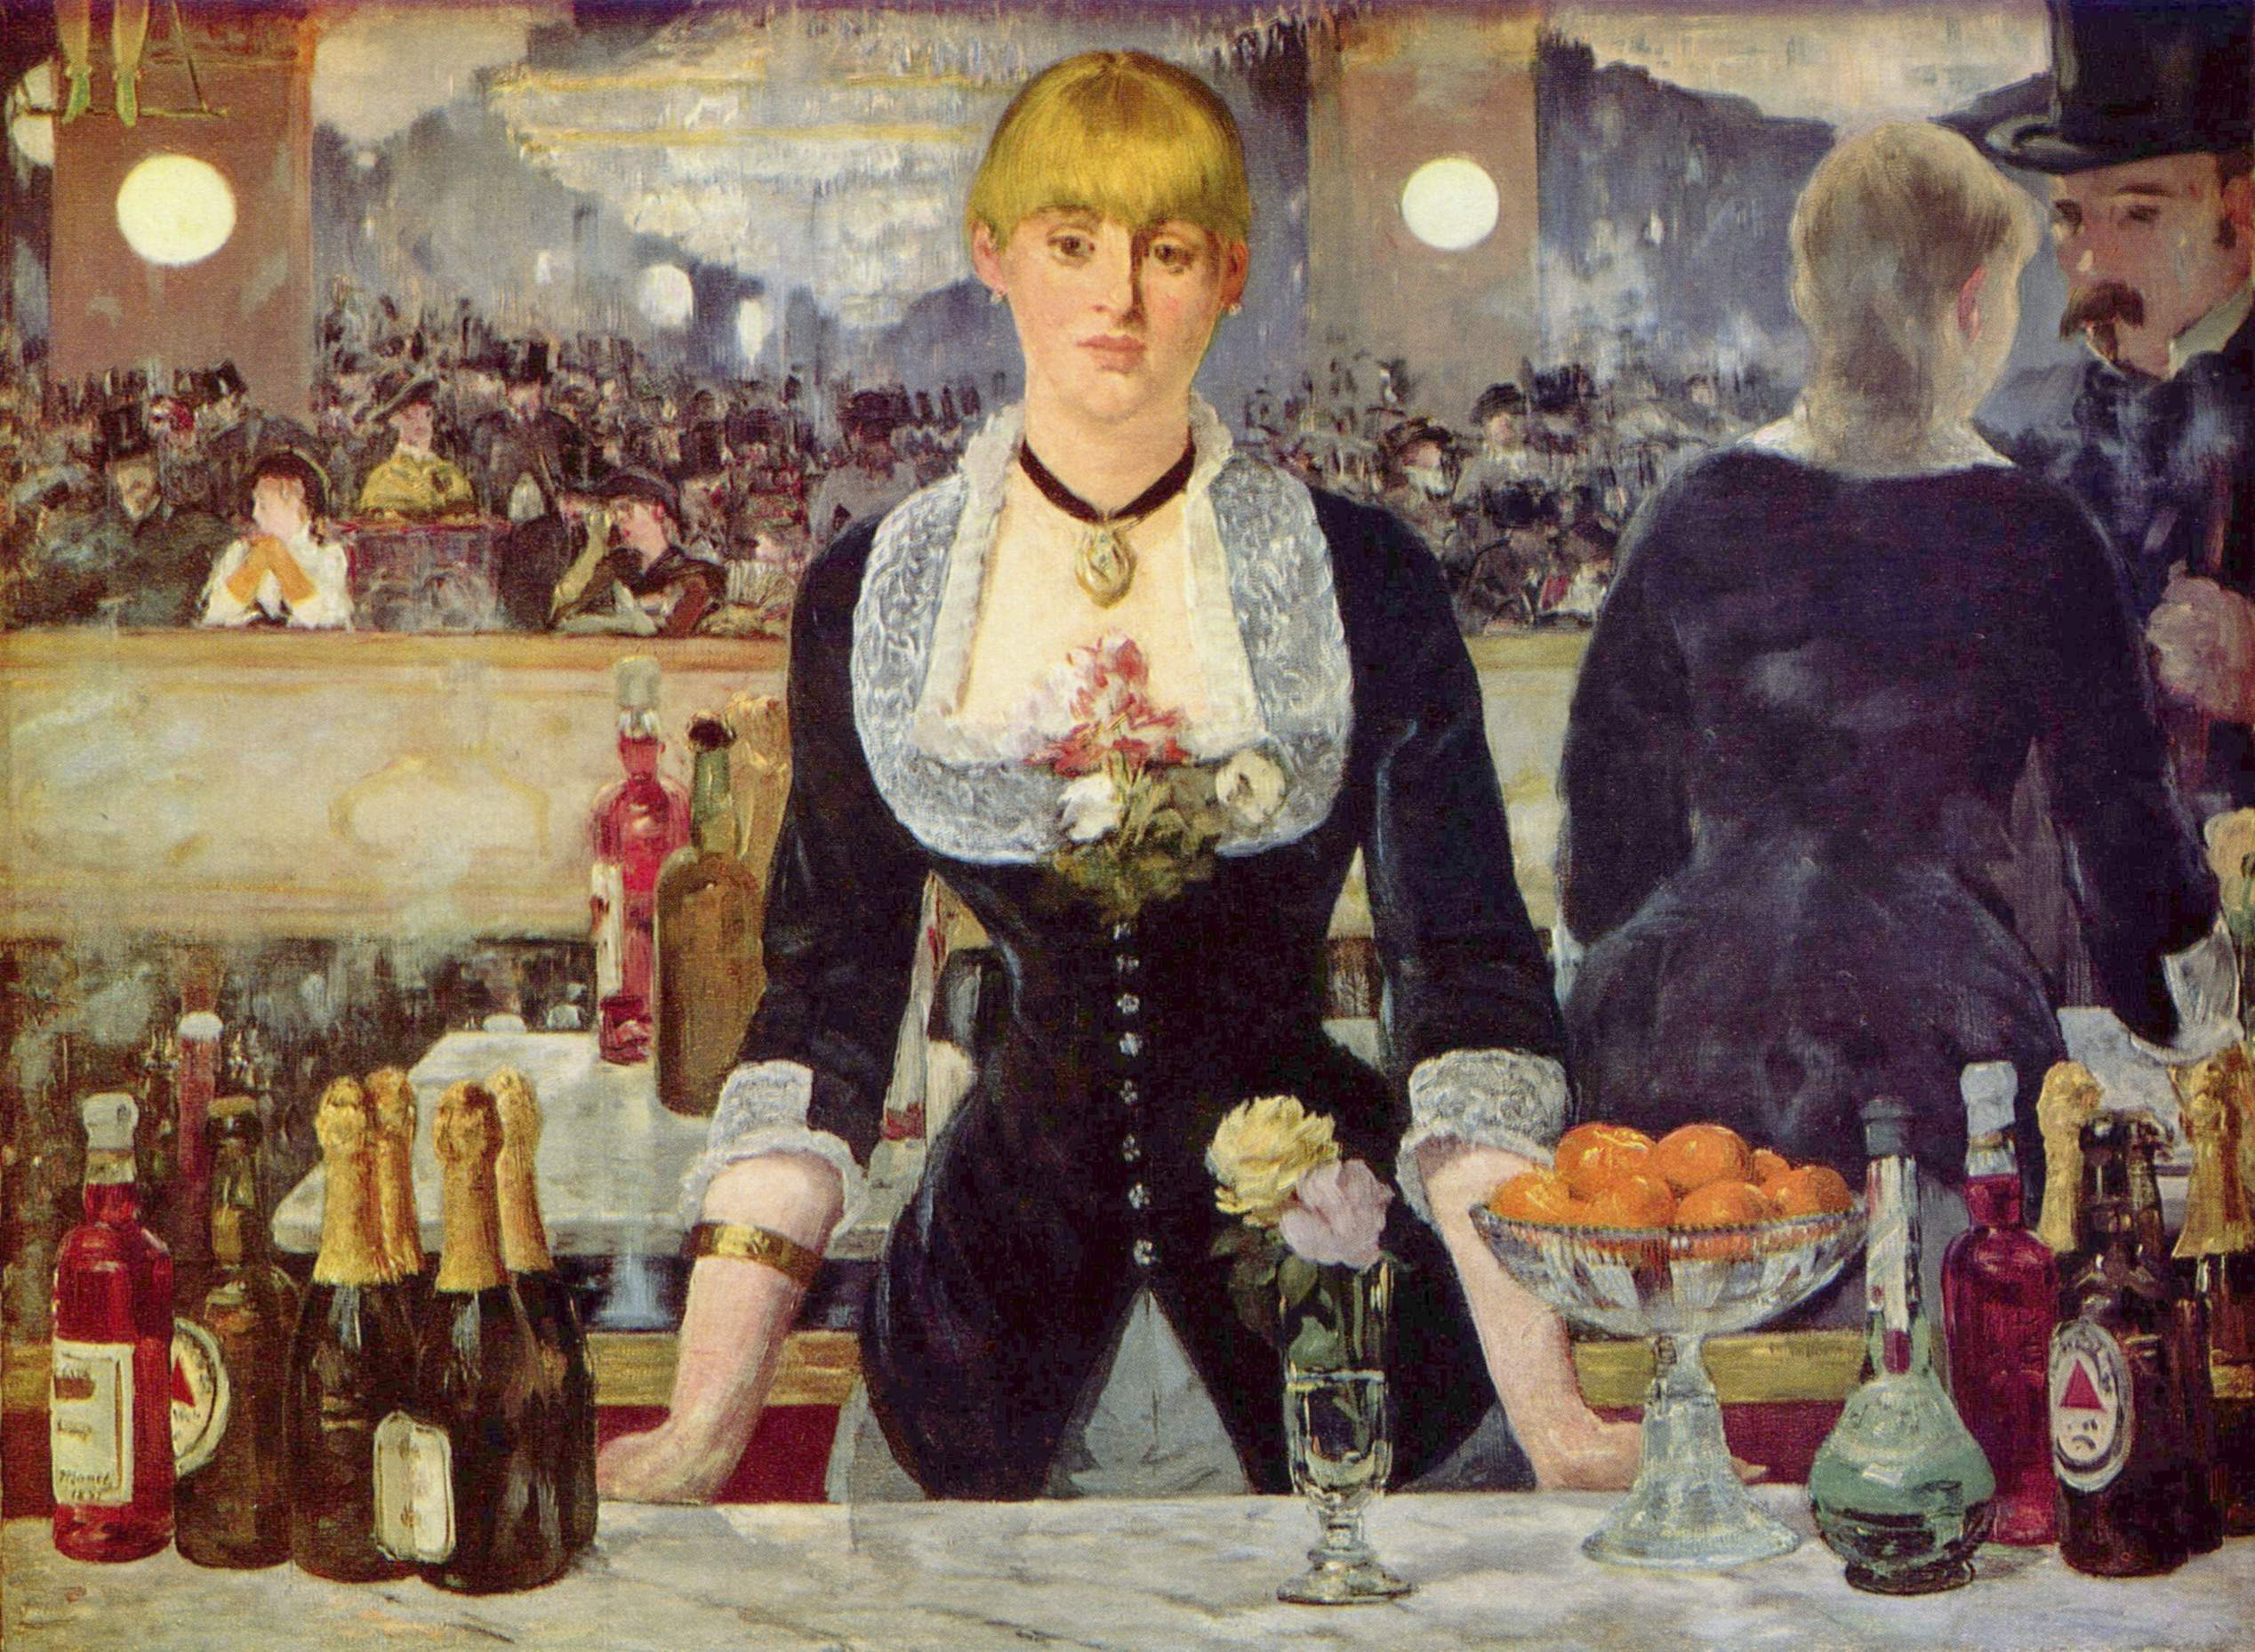
\includegraphics[width=1.1\textwidth]{manet}\par
    \par\hfill\hfill{\tiny\bfseries Man\`et  \textit{The Barmaid.}}\\
    \par
    \vspace*{\baselineskip}
    \par
    \begin{center}
    \noindent\large\bfseries EDOUARD MANET
    \end{center}
    \begin{multicols}{3}
      \leftskip0pt
      \lettrine[lines=2]{I}{psum dolor} sit amet latixeus. \lipsum*[1-2]
      Latinicus porcupinus to fill the line.
    \end{multicols}
% \end{minipage}
\clearpage
\end{document}